%!TEX root = ../../super_main.tex

\section{Participant Interaction}

% Initial screen
\begin{figure}
\begin{subfigure}[!t]{\textwidth}
  \centering
  
\includegraphics[width=.4\linewidth]{mockups/homepage}
  \caption{Mockup.}
  \label{fig:mockup_initial_screen}
\end{subfigure}

\begin{subfigure}[!t]{.52\textwidth}
  \centering
  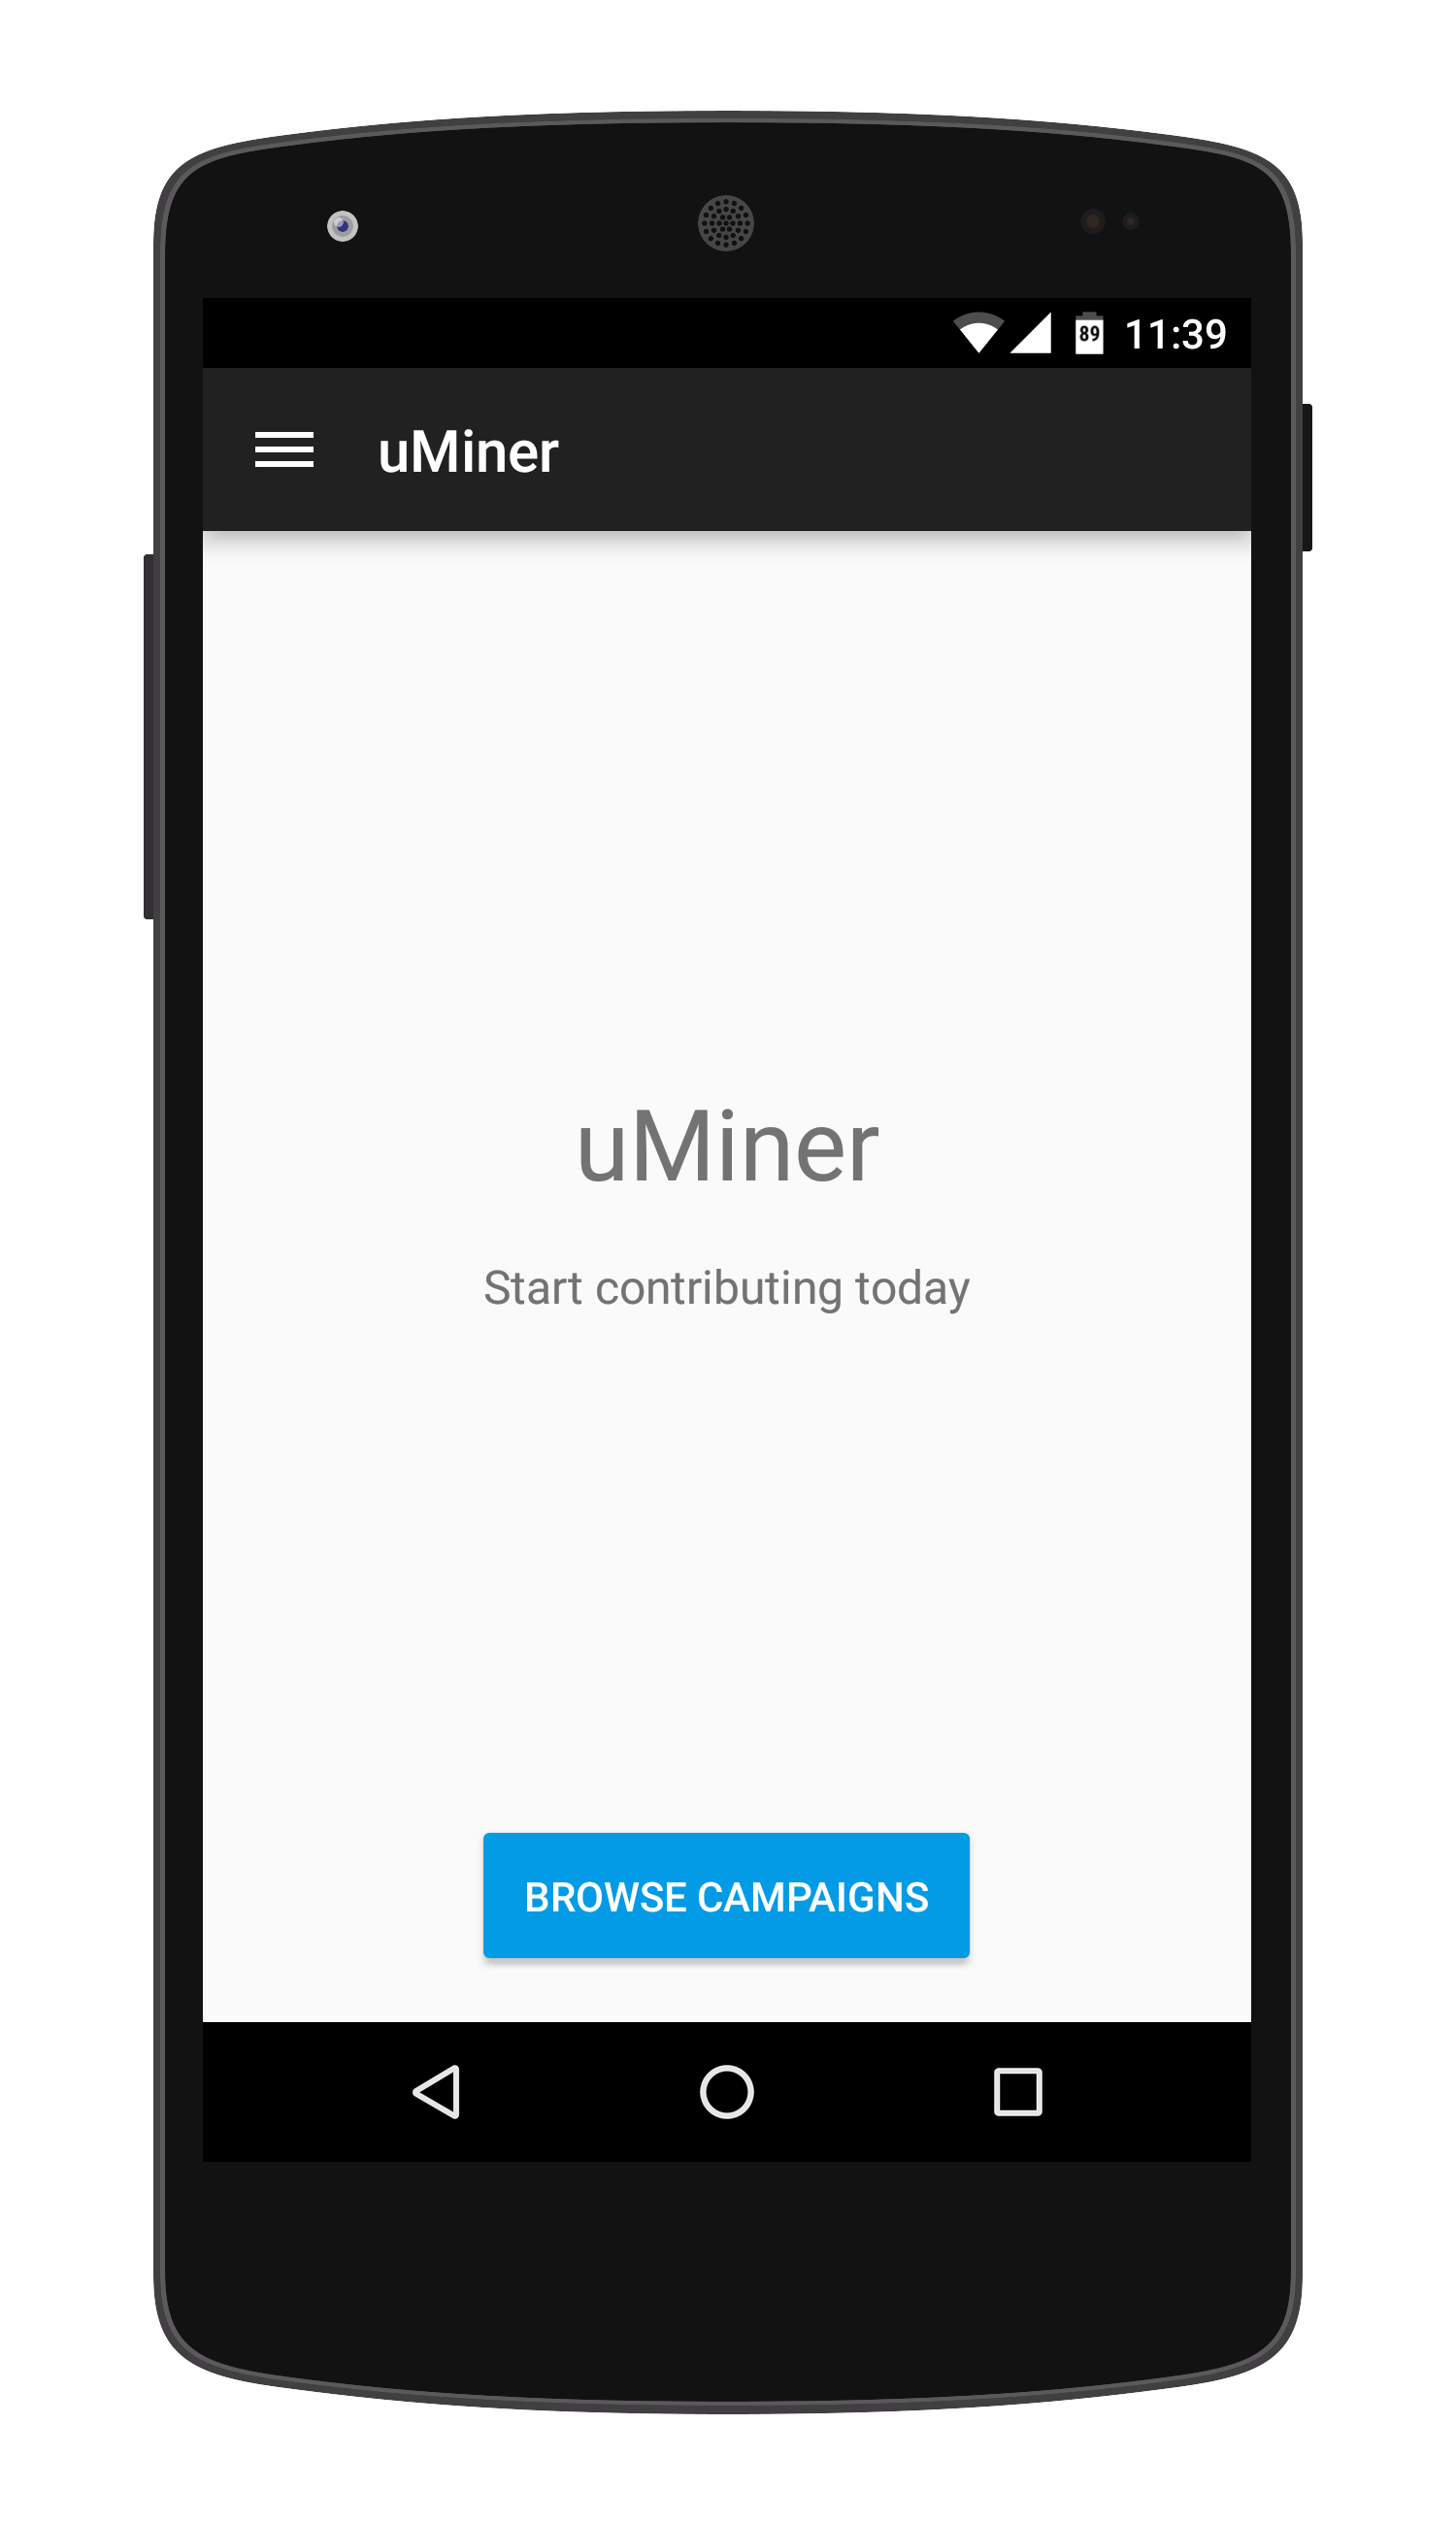
\includegraphics[width=.82\linewidth]{user_interfaces/client_uminer_home_with_phone}
  \caption{Implementation.}
  \label{fig:implementation_initial_screen}
\end{subfigure}%
\begin{subfigure}[!t]{.52\textwidth}
  \centering
  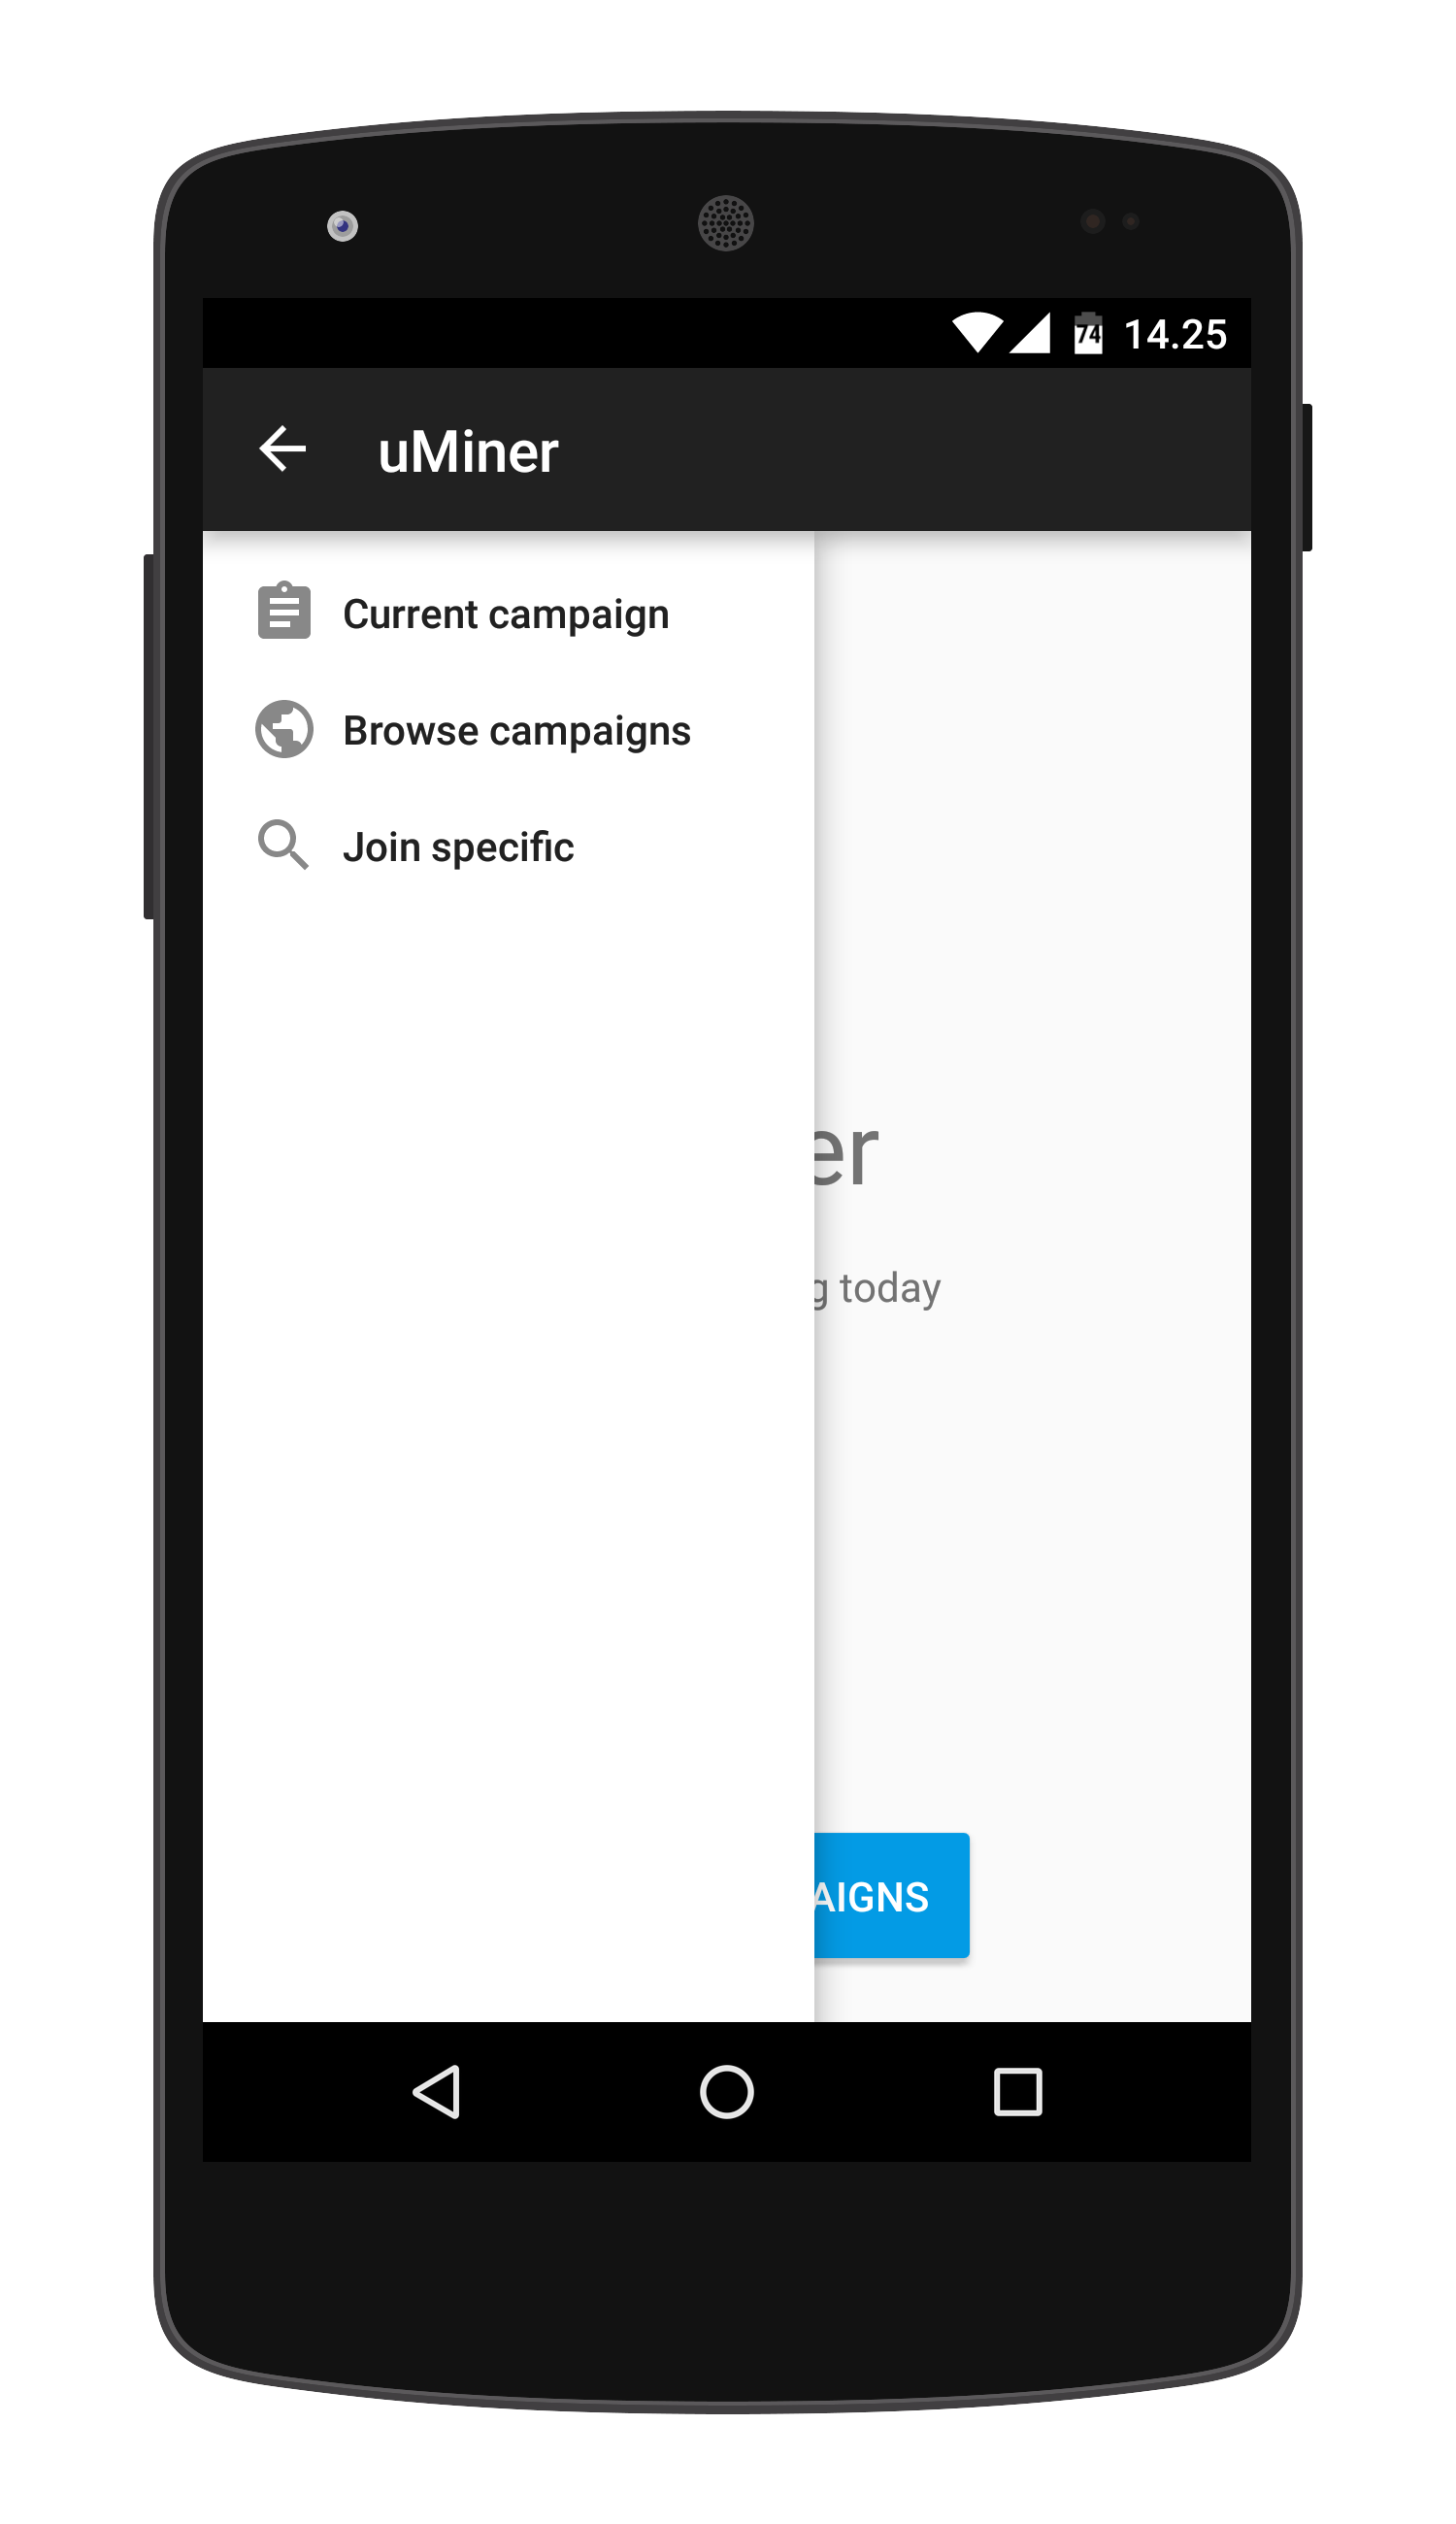
\includegraphics[width=.82\linewidth]{user_interfaces/client_drawer_menu_with_phone}
  \caption{Drawer menu supporting navigation.}
  \label{fig:drawer_menu}
\end{subfigure}
\caption{Campaign specifications.}
\label{fig:initial_screen}
\end{figure}
\FloatBarrier

% Publicly available campaigns
\begin{figure}
\begin{subfigure}[!t]{.48\textwidth}
  \centering
  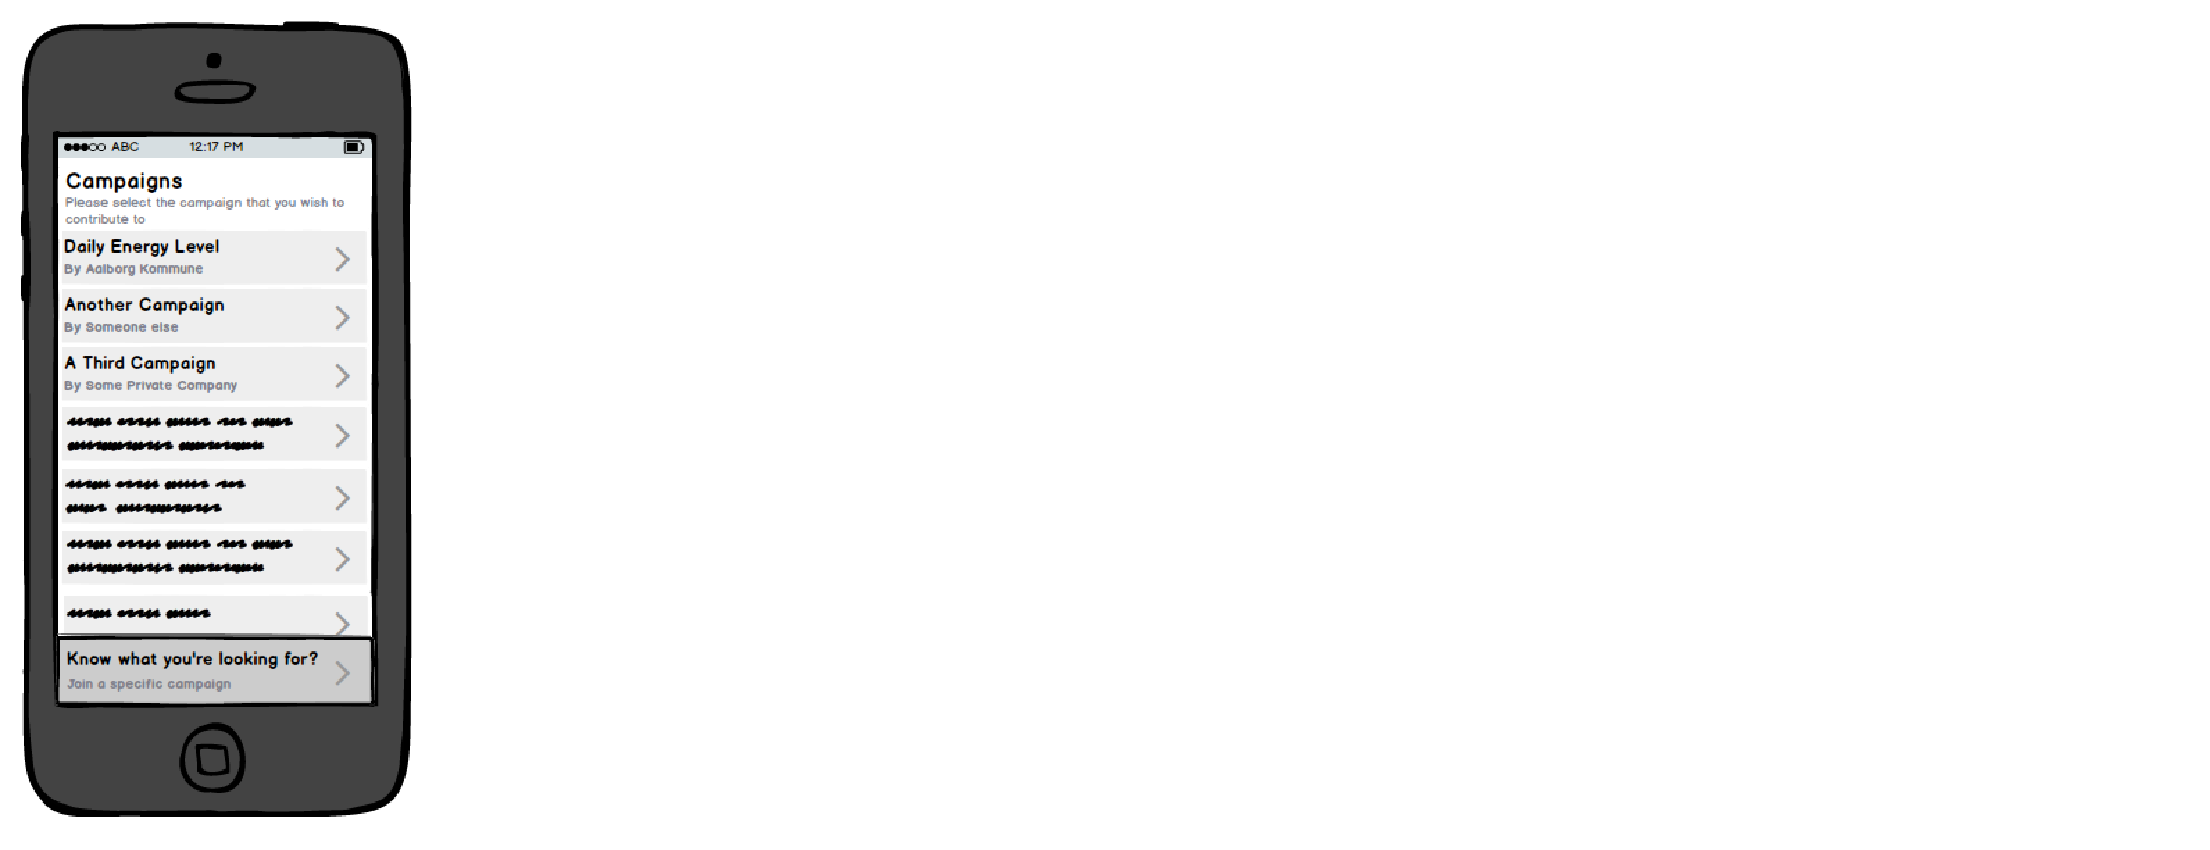
\includegraphics[width=.8\linewidth]{mockups/campaigns_list}
  \caption{Mockup.}
  \label{fig:mockup_public_campaigns}
\end{subfigure}%
\begin{subfigure}[!t]{.52\textwidth}
  \centering
  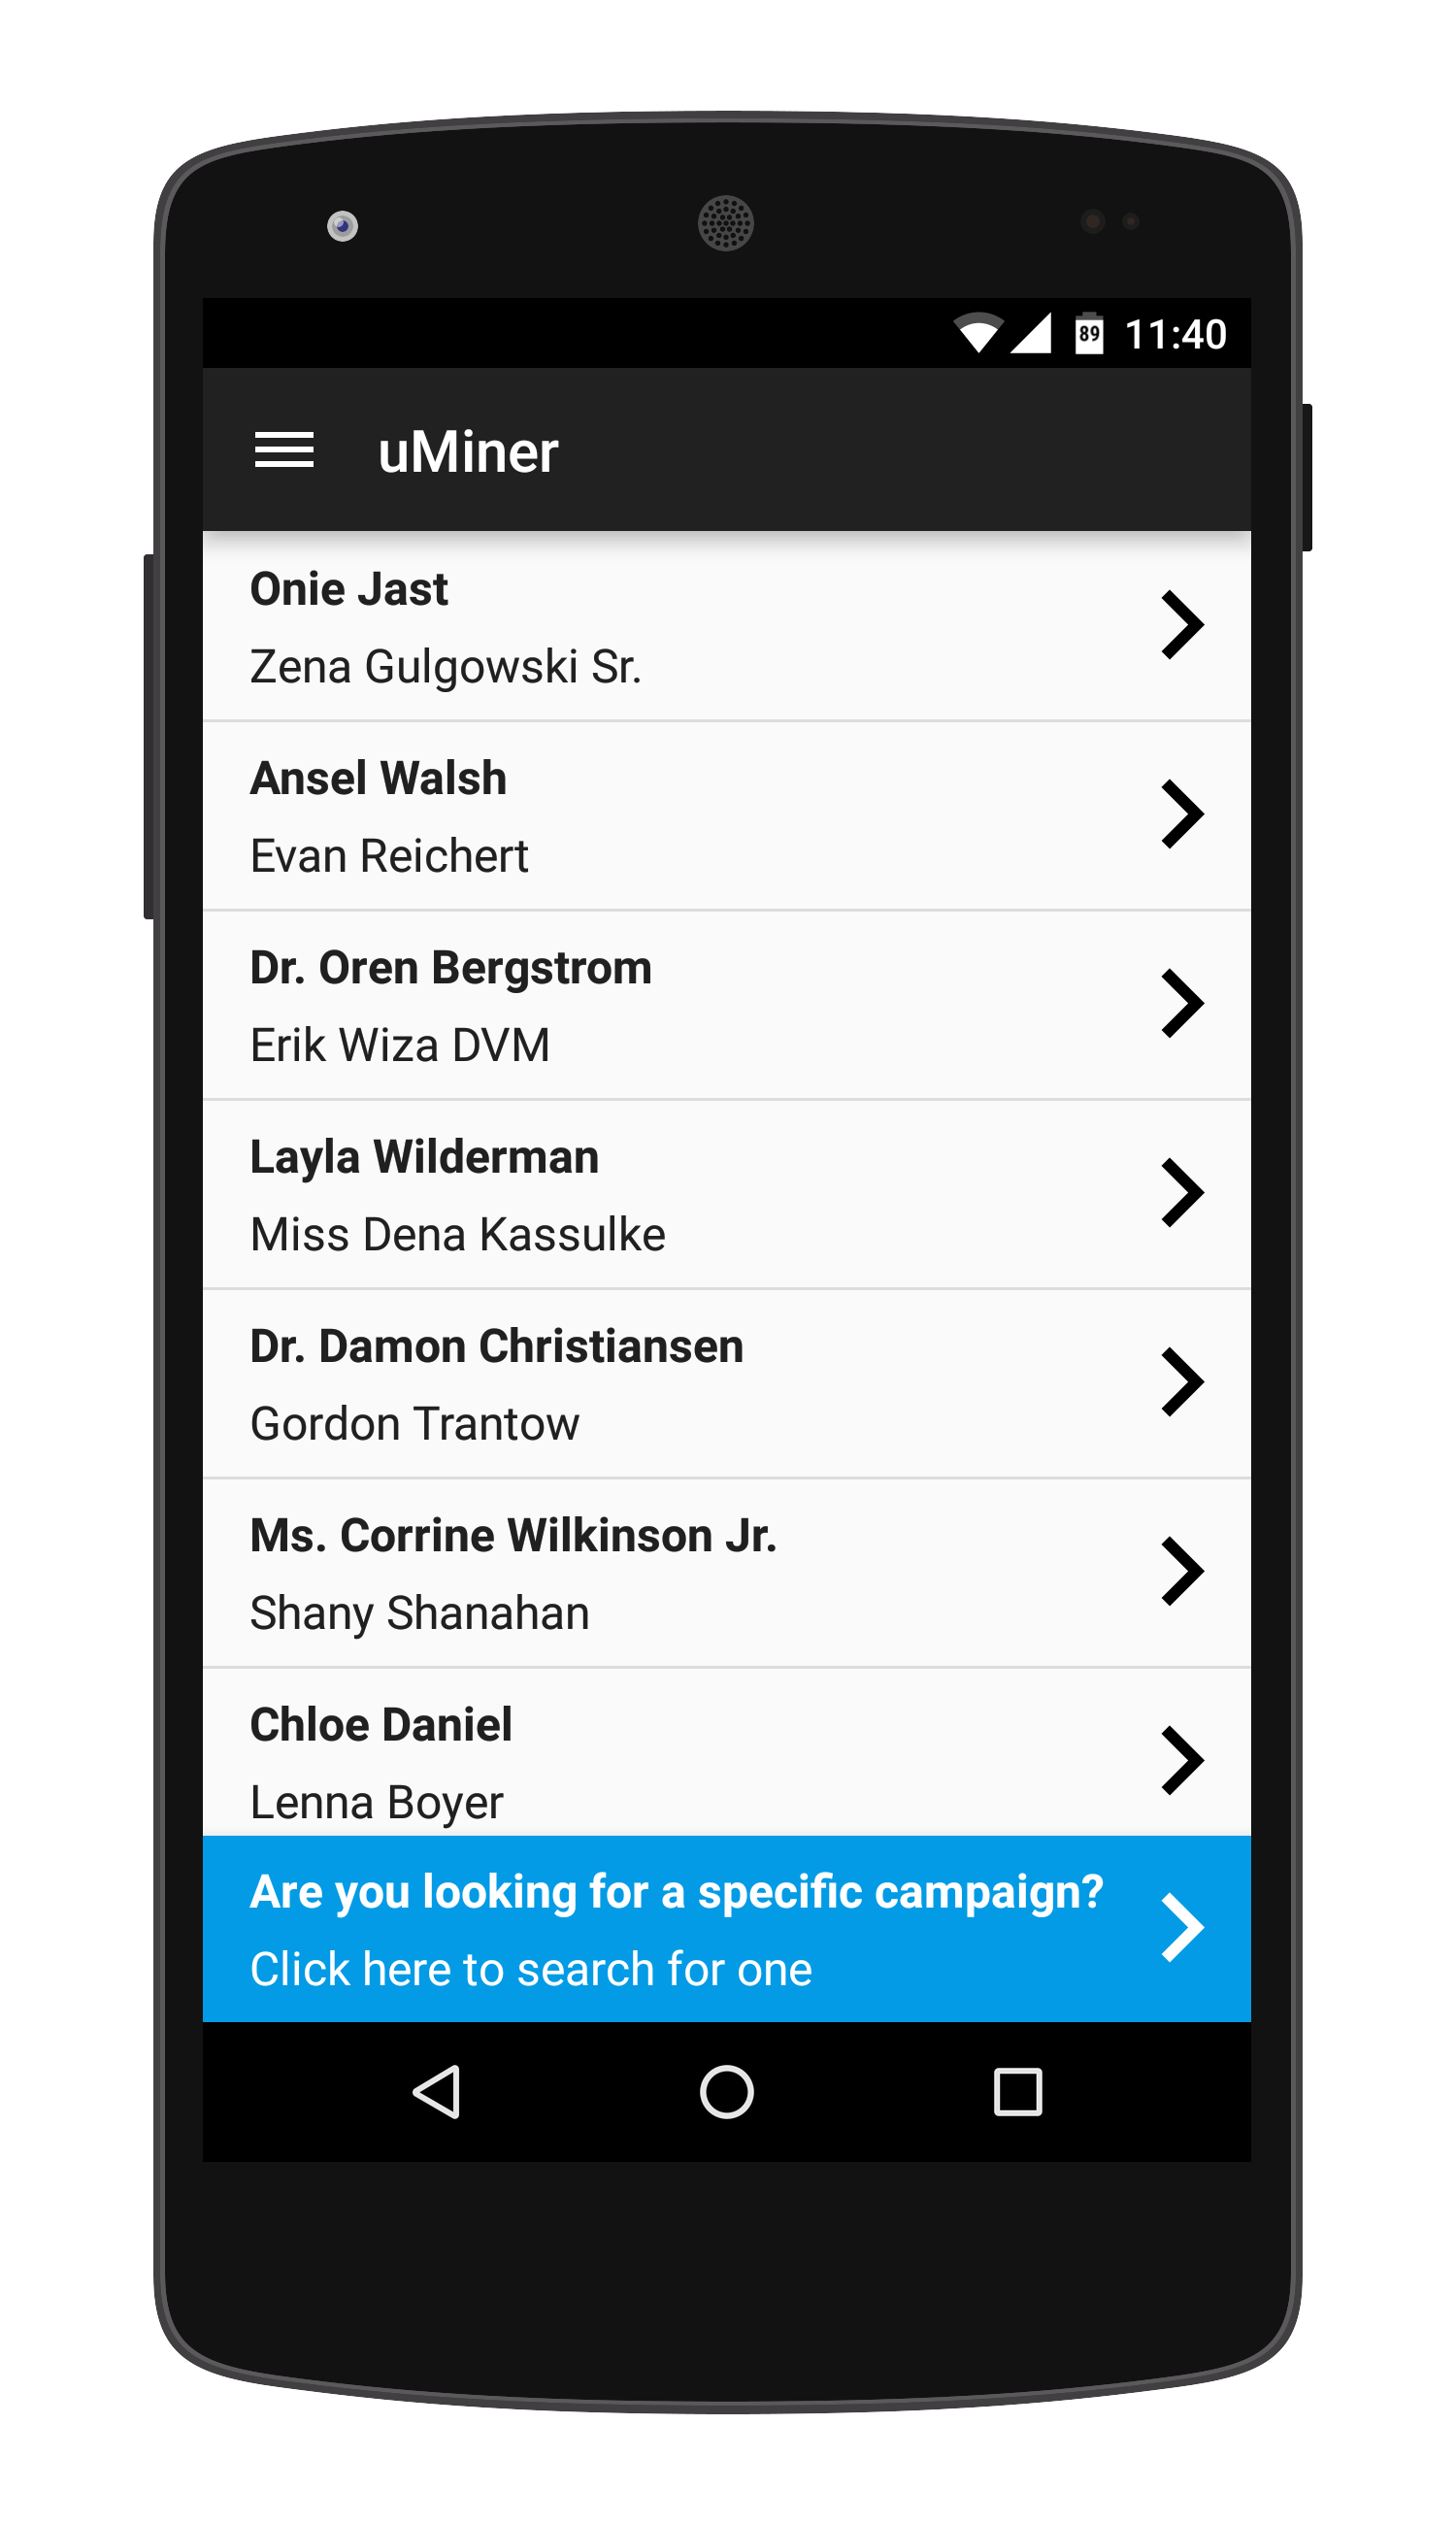
\includegraphics[width=.83\linewidth]{user_interfaces/client_public_campaigns_with_phone}
  \caption{Implementation.}
  \label{fig:implementation_public_campaigns}
\end{subfigure}
\caption{List of publicly available campaigns.}
\label{fig:public_campaigns}
\end{figure}
\FloatBarrier

% Search for a campaign through a campaign identifier
\begin{figure}
\begin{subfigure}[!t]{.48\textwidth}
  \centering
  
\includegraphics[width=.8\linewidth]{mockups/join_specific_campaign}
  \caption{Mockup.}
  \label{fig:mockup_specific_campaign}
\end{subfigure}%
\begin{subfigure}[!t]{.52\textwidth}
  \centering
  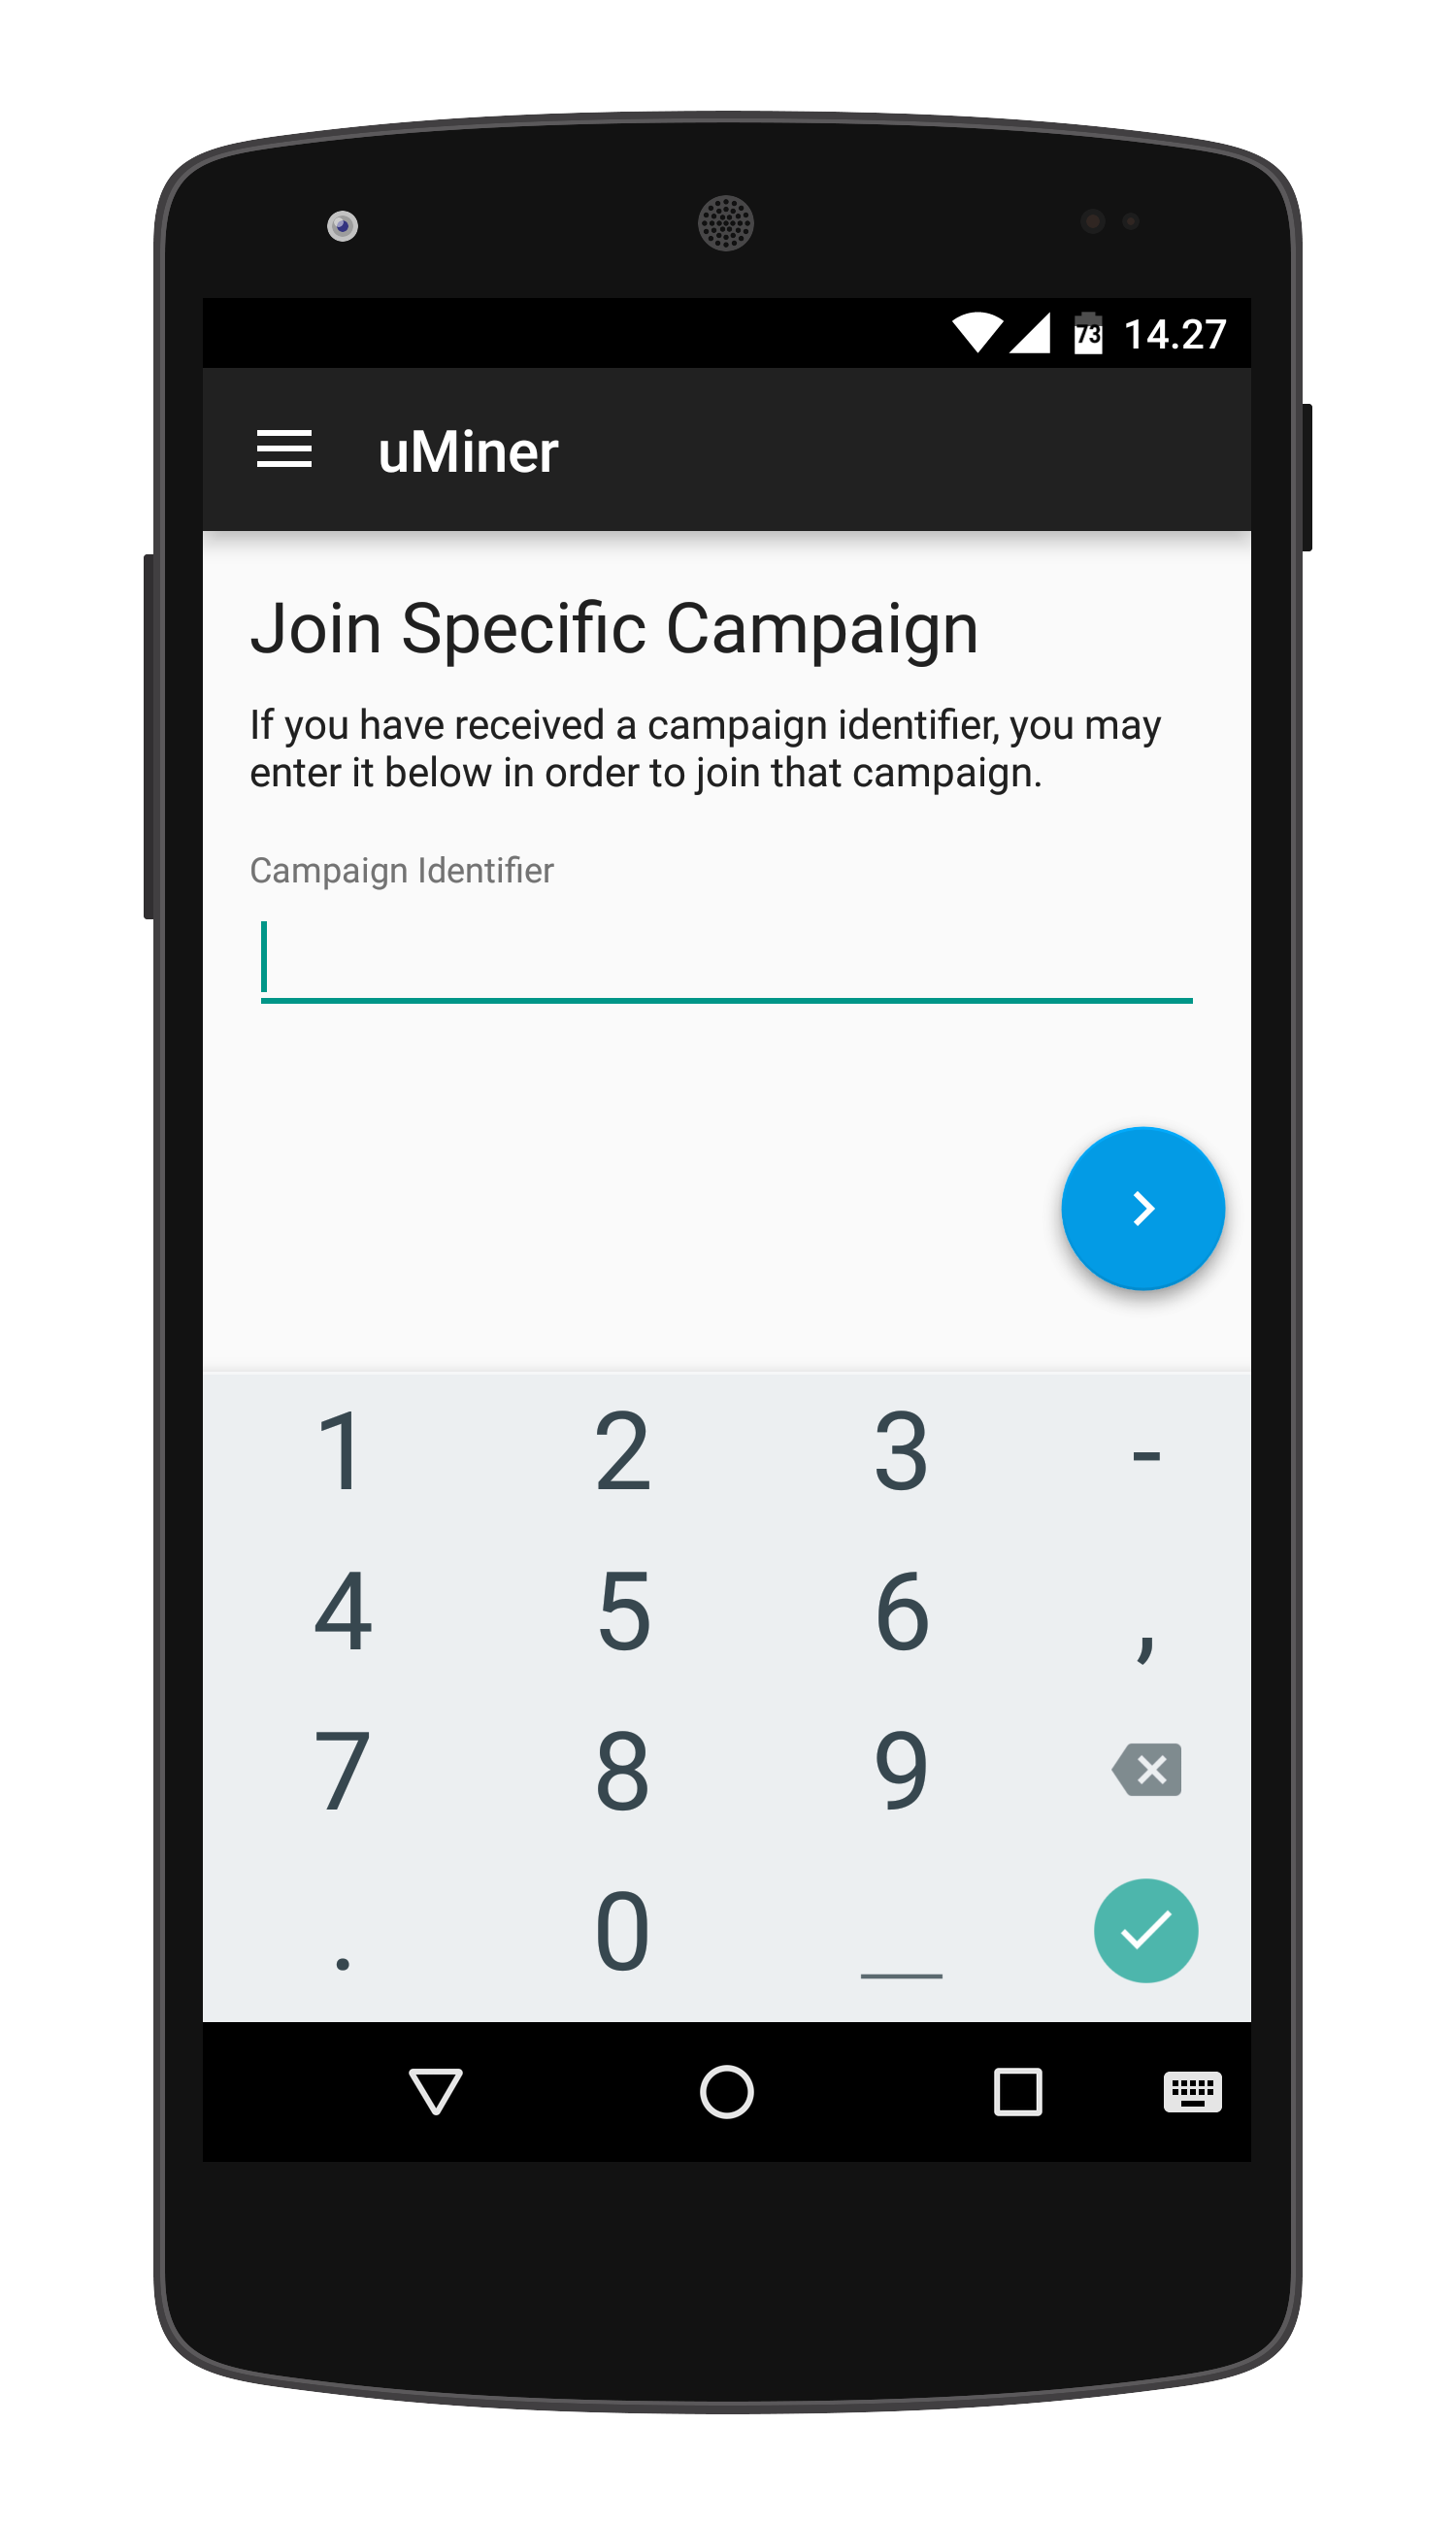
\includegraphics[width=.83\linewidth]{user_interfaces/client_join_specific_campaign_with_phone}
  \caption{Implementation.}
  \label{fig:implementation_specific_campaign}
\end{subfigure}
\caption{Search for a specific campaign using a campaign identifier.}
\label{fig:specific_campaign}
\end{figure}
\FloatBarrier

% Search for a campaign through a campaign identifier
\begin{figure}
\begin{subfigure}[!t]{.48\textwidth}
  \centering
  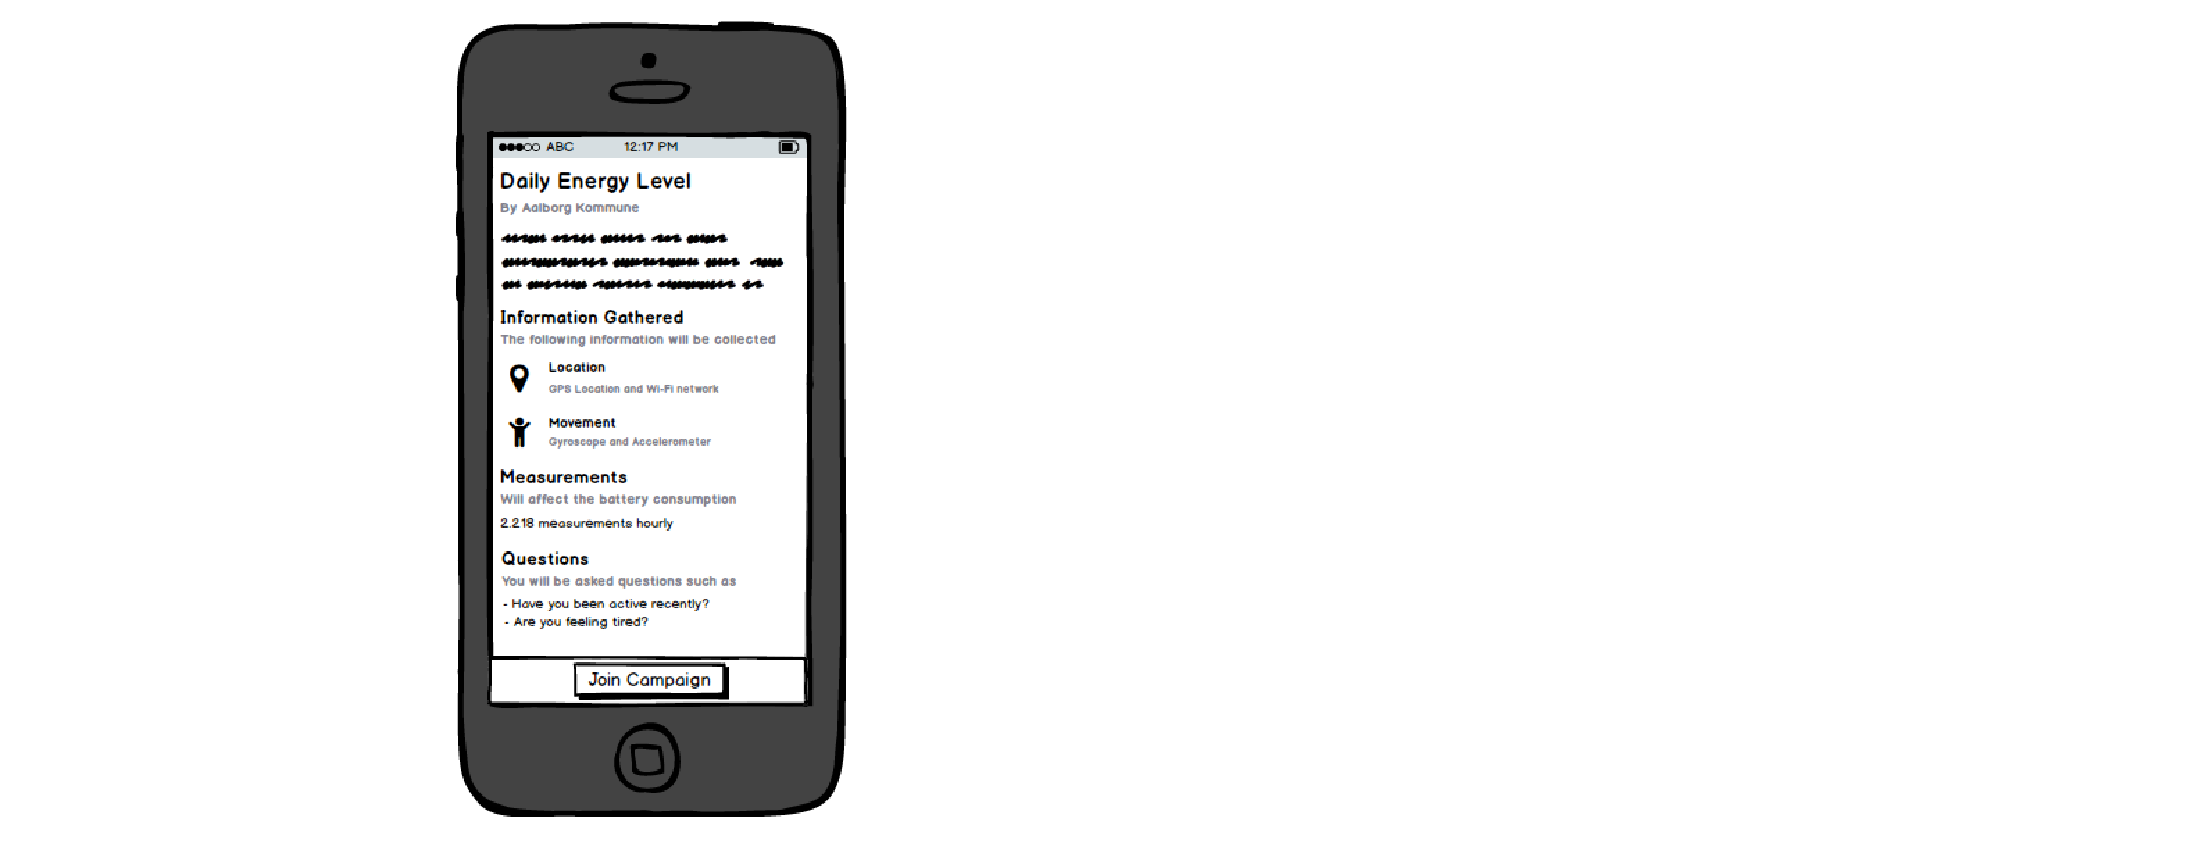
\includegraphics[width=.8\linewidth]{mockups/campaign_specification}
  \caption{Mockup.}
  \label{fig:mockup_campaign_specification}
\end{subfigure}%
\begin{subfigure}[!t]{.52\textwidth}
  \centering
  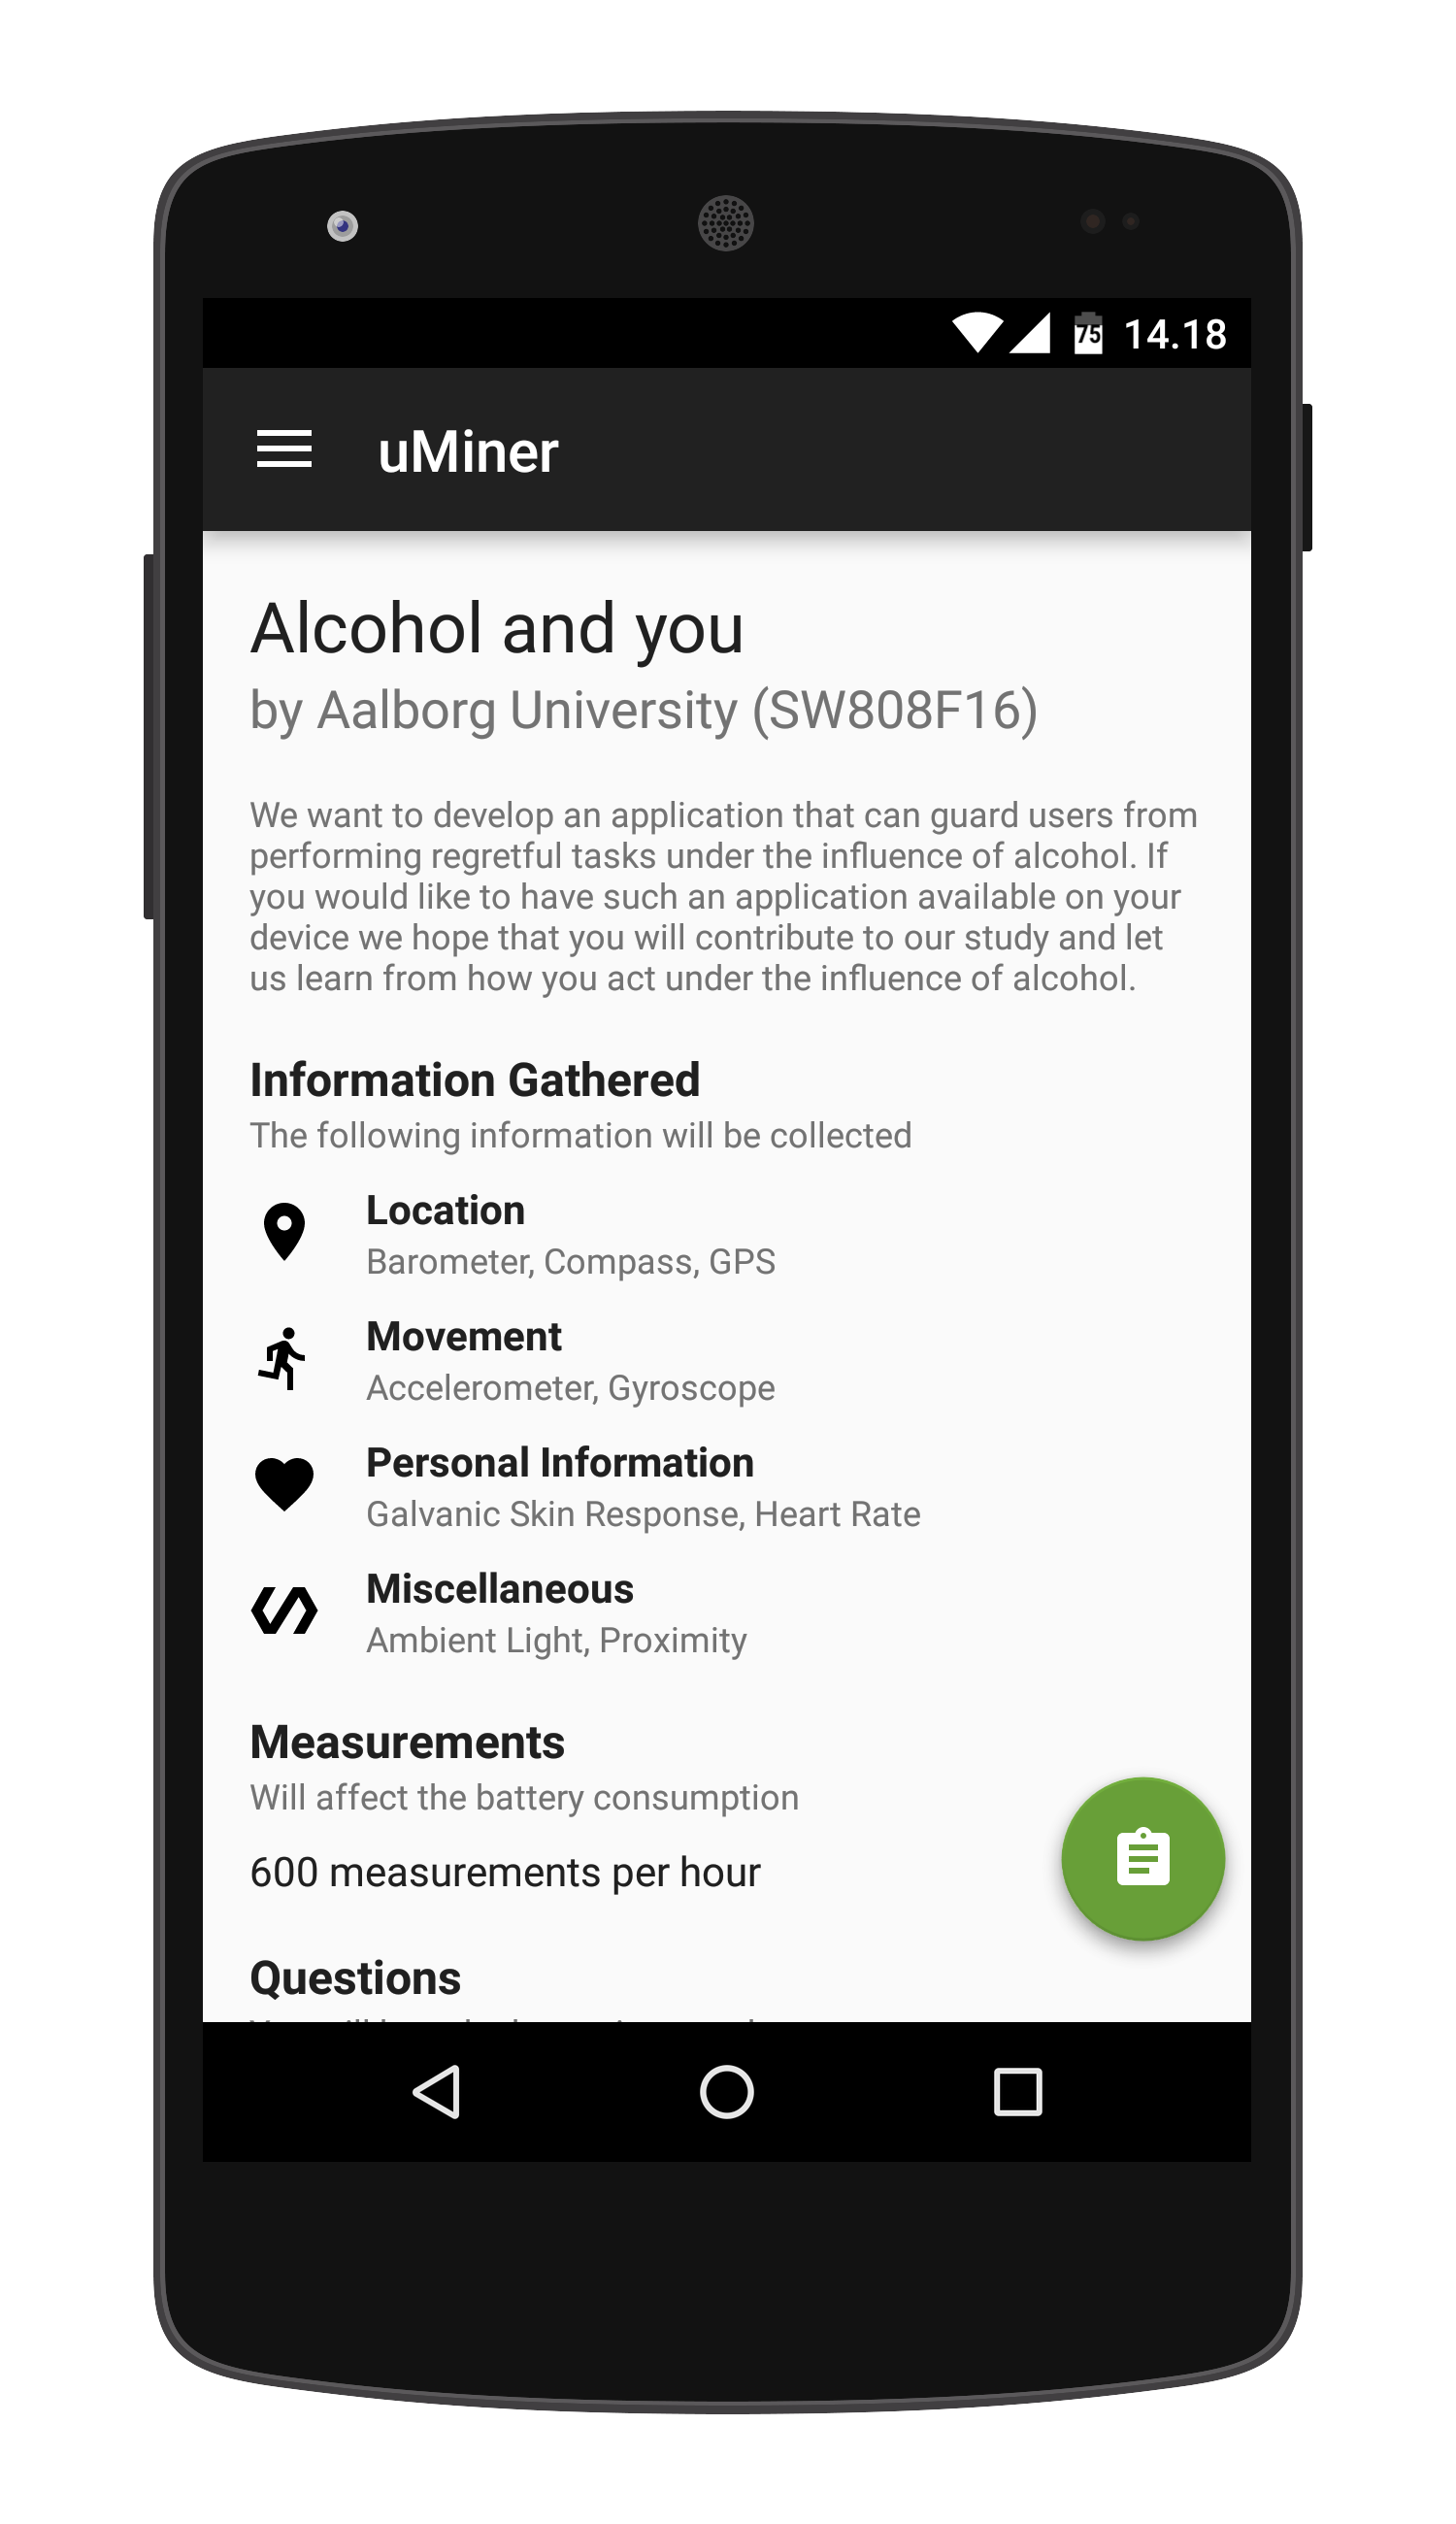
\includegraphics[width=.83\linewidth]{user_interfaces/client_campaign_specification2_with_phone}
  \caption{Implementation.}
  \label{fig:implementation_campaign_specification}
\end{subfigure}
\caption{Campaign specification view.}
\label{fig:campaign_specification}
\end{figure}
\FloatBarrier